%----------------------------------------------------------------------------
\chapter{Tervezés és megvalósítás}
%----------------------------------------------------------------------------

A rendszer architektúrájának tervezése során figyelembe vettem a \ref{research}. és \ref{scopes}. fejezetekben kitűzött célokat. Az eretedi tervek elkészültével kezdetét vette a megvalósítás. Az implementáció során felmerültek olyan akadályok és újabb ötletek, amelyek kisebb-nagyobb mértékben befolyásolták a terveket. Erre számítottam és éppen ezért úgy próbáltam tervezni, hogy dinamikusan módosíthatóak legyenek és bővítés vagy módosítás esetén. A tervezési és megvalósítási folyamat hónapokat vedd igénybe annak érdekében, hogy minden jelentkező problémát és az újabb ötleteket legyen idő átgondolni.

\section {Az alkalmazás frontendje}

\subsection {Kezdőoldal (Homepage)}

Tekintettel arra, hogy az alkalmazás bizonyos funkcionalitásai használhatóak bejelentkezés nélkül is, a kezdőoldal egy üdvözlő oldal egy navigációs menüvel az oldal tetején. Amennyiben egy eszközről első alkalommal lépik az oldalra egy felhasználó, akkor egy információs ablakkal találkozik \cite{Modal}, amely tartalmazza az alkalmazás célját, a hivatalos forrásokat a jegyvásárlásra és ezeknek a jogtulajdonosait (\ref{abra:homepagePopup}).

Annak érdekében, hogy ez az ablak csak egyszer jelenleg meg \textbf{sütiket (Cookies)} használok. Ezek a sütiket a böngésző tárolja a felhasználó eszközén és a weboldal betöltésekor a böngésző betölti az elmentett sütiket, ha vannak. Ezek kulcs-elem párok, amely értelmében egy tetszőleges nevű kulcs alatt tudok elmenteni majdnem bármilyen adatot. Ha a felhasználó rákattint az \textbf{Understood} gombra, akkor egy \textbf{modalAccepted} kulcs alatti sütiben eltárolom a \textbf{true} értéket és amikor betöltődik az alkalmazás ezt az értéket ellenőrzöm.
Mint említettem ezek a sütik lokálisan vannak tárolva a felhasználónál és ha a felhasználó kitörli azokat, amelyek ehhez az oldalhoz tartoznak, akkor egyértelműen újra elő fog jönni egy az ablak.

\begin{figure}[!h]
	\centering
	
\includegraphics[scale=0.4]{images/homepagePopup}
	\caption{Kezdőoldalon felugró ablak}
	\label{abra:homepagePopup}
\end{figure}
\pagebreak

\begin{figure}[!h]
	\centering
	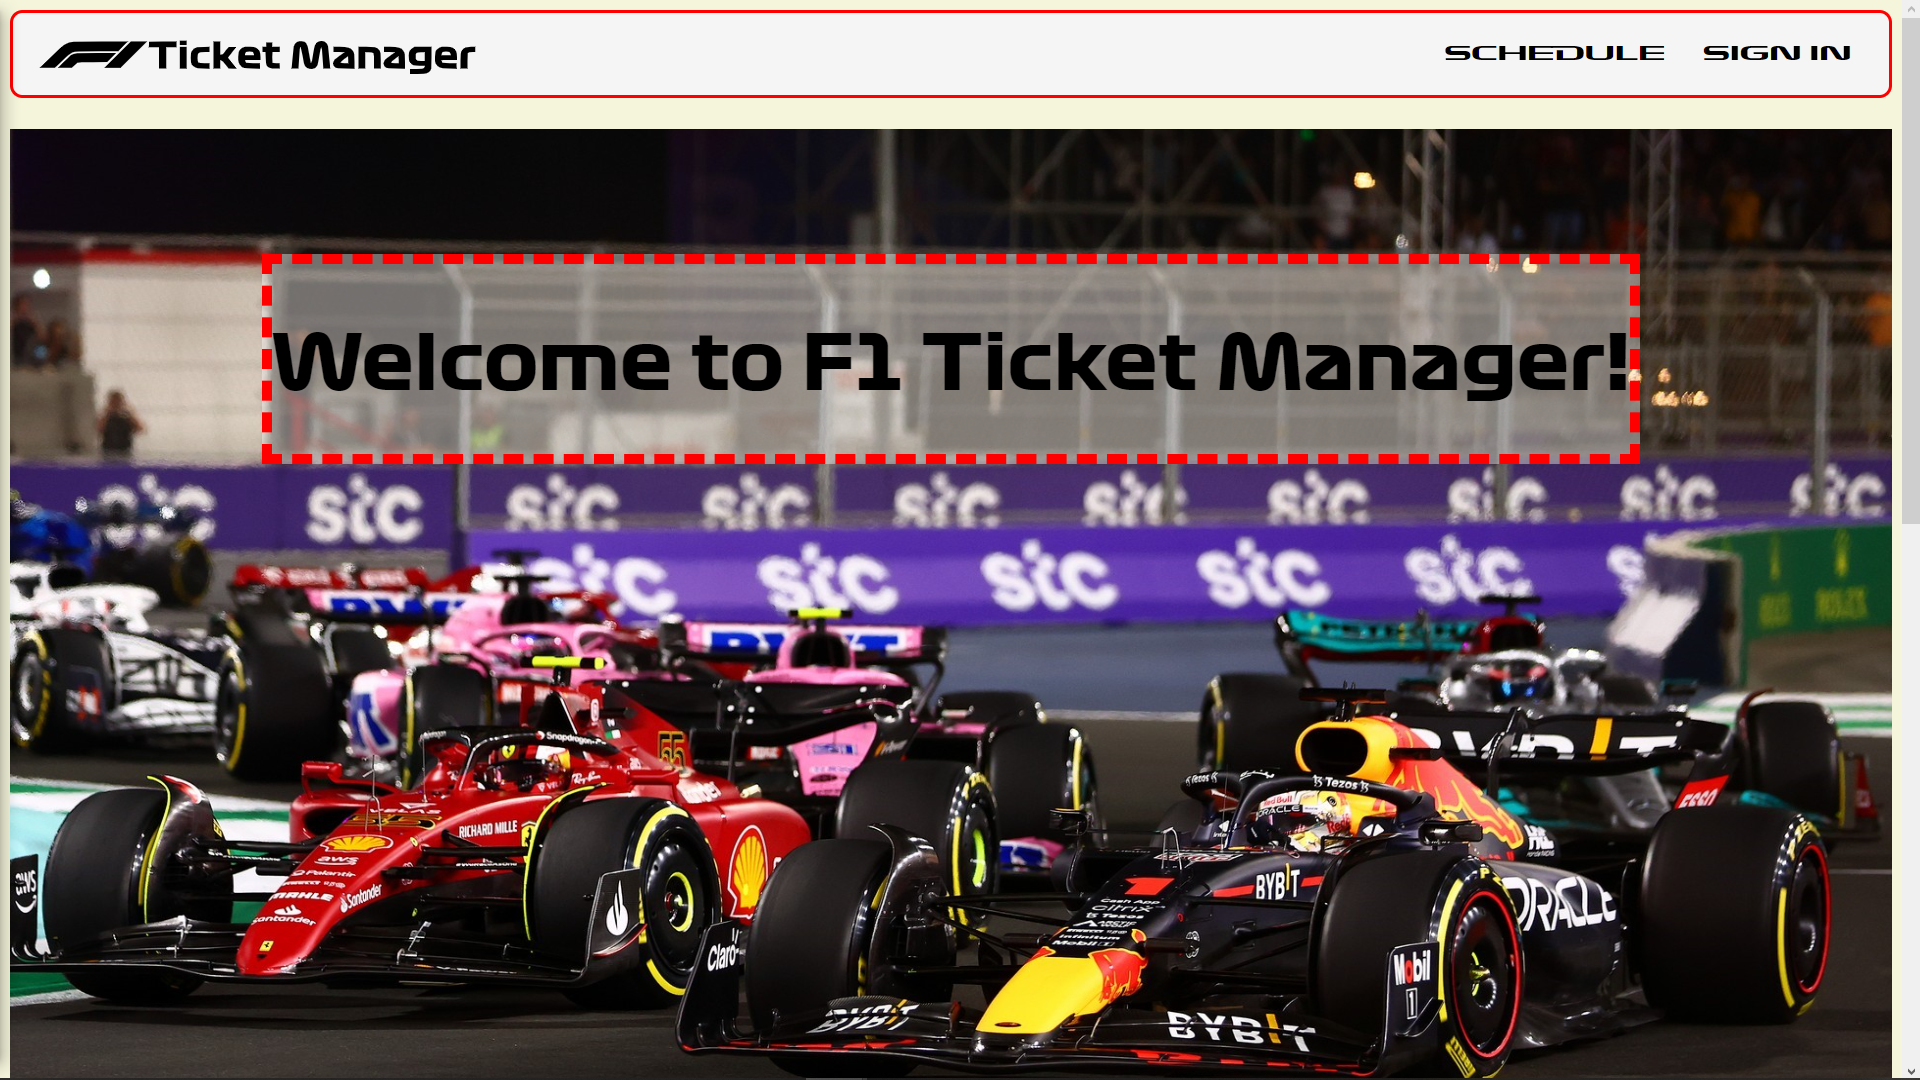
\includegraphics[scale=0.2]{images/homepage}
	\caption{Kezdőoldal}
	\label{abra:homepage}
\end{figure}
\pagebreak

\subsection {Versenynaptár (Schedule)}

A \textbf{Versenynaptár} oldalon lehet böngészni a 2022-es év versenyeinek listáját a megrendezési sorrendben. Az első kártya, ami megjelenik az oldalon az a következő verseny, amely automatikusan kerül ki az aktuális dátum alapján. Teszt jelleggel van egy dátum kiválasztó gomb is, hogy ki lehessen próbálni, hogy egy adott dátumhoz melyik verseny lesz a legközelebb. Erre a kártyára kattintva meg lehet tekinteni a részleteket. Minden kártyán látszanak a legfontosabb információk az adott versenyről, mint a pálya neve, a rendező ország neve, az intervallum, amikor az esemény zajlani fog és a pályarajz (\ref{abra:schedule}).

\begin{figure}[!h]
	\centering
	\begin{tabular}{cc}
	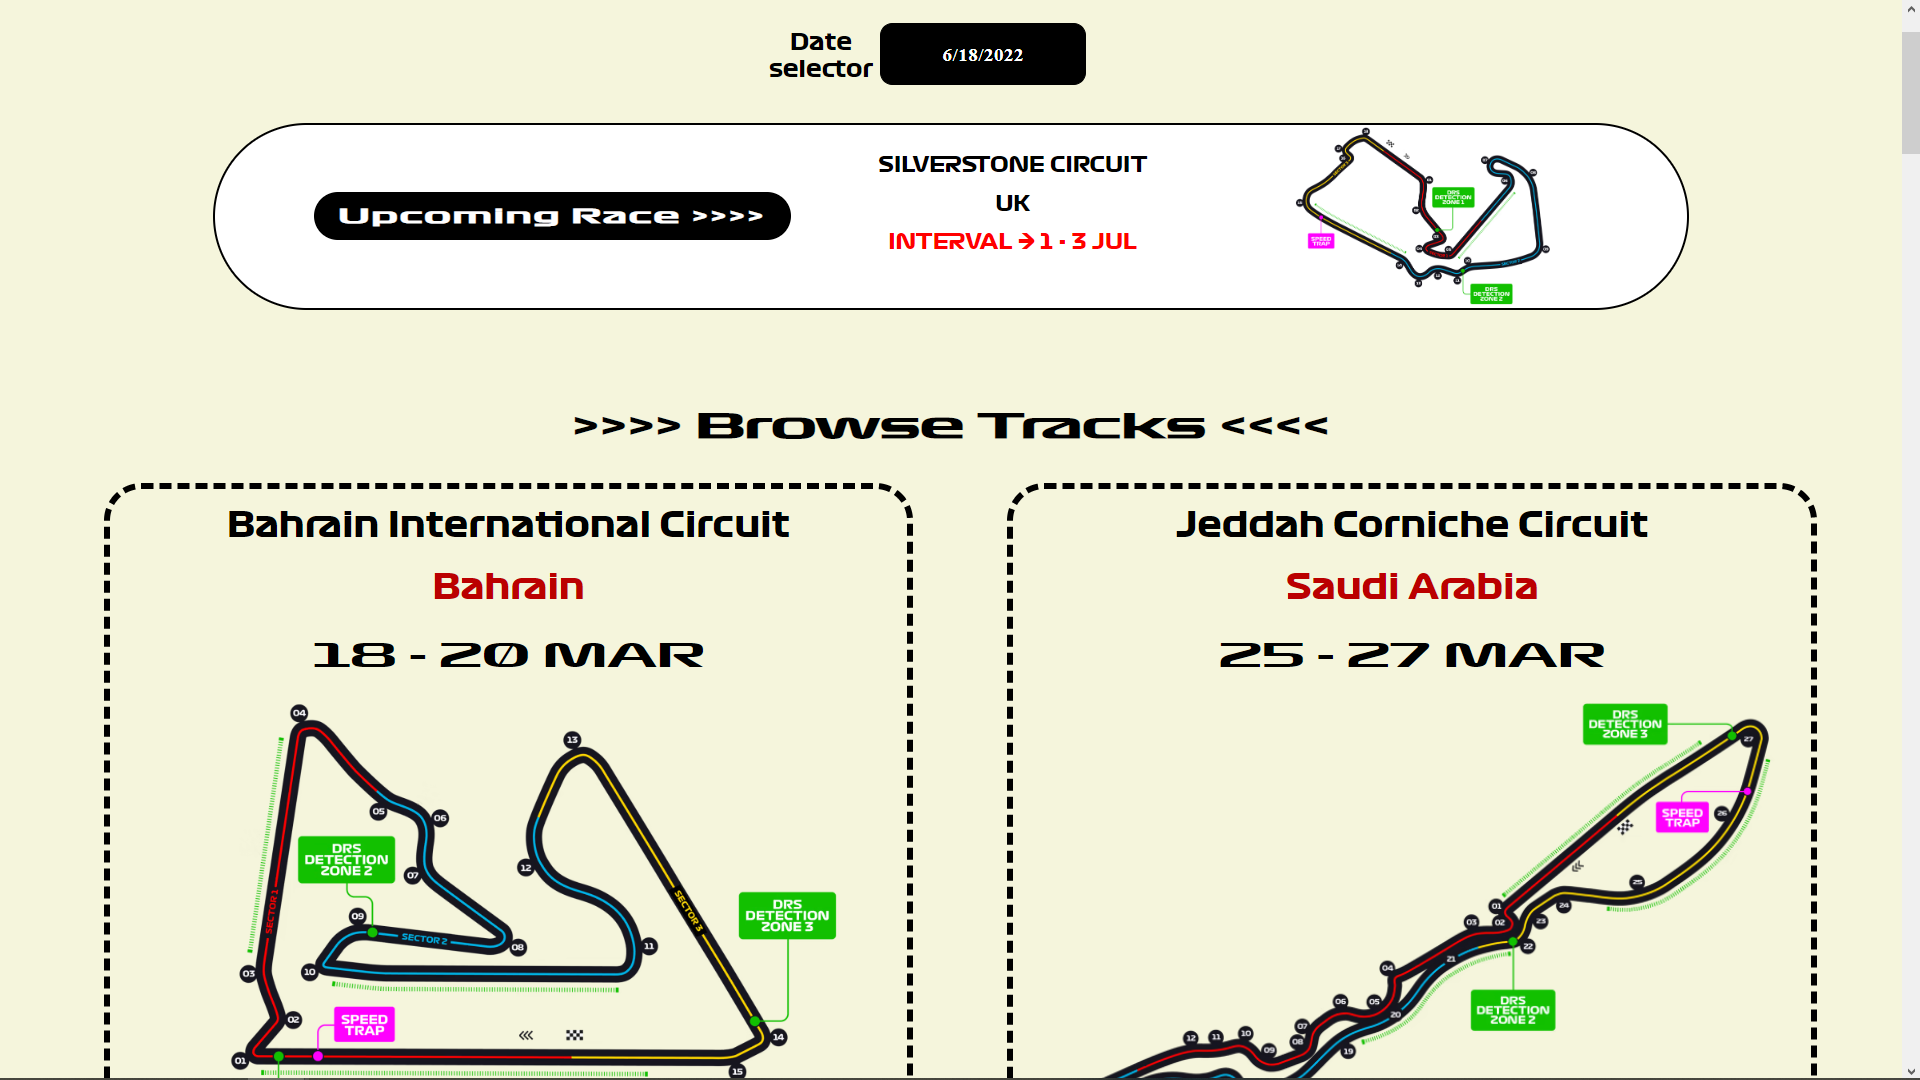
\includegraphics[scale=0.15]{images/schedule1} &
	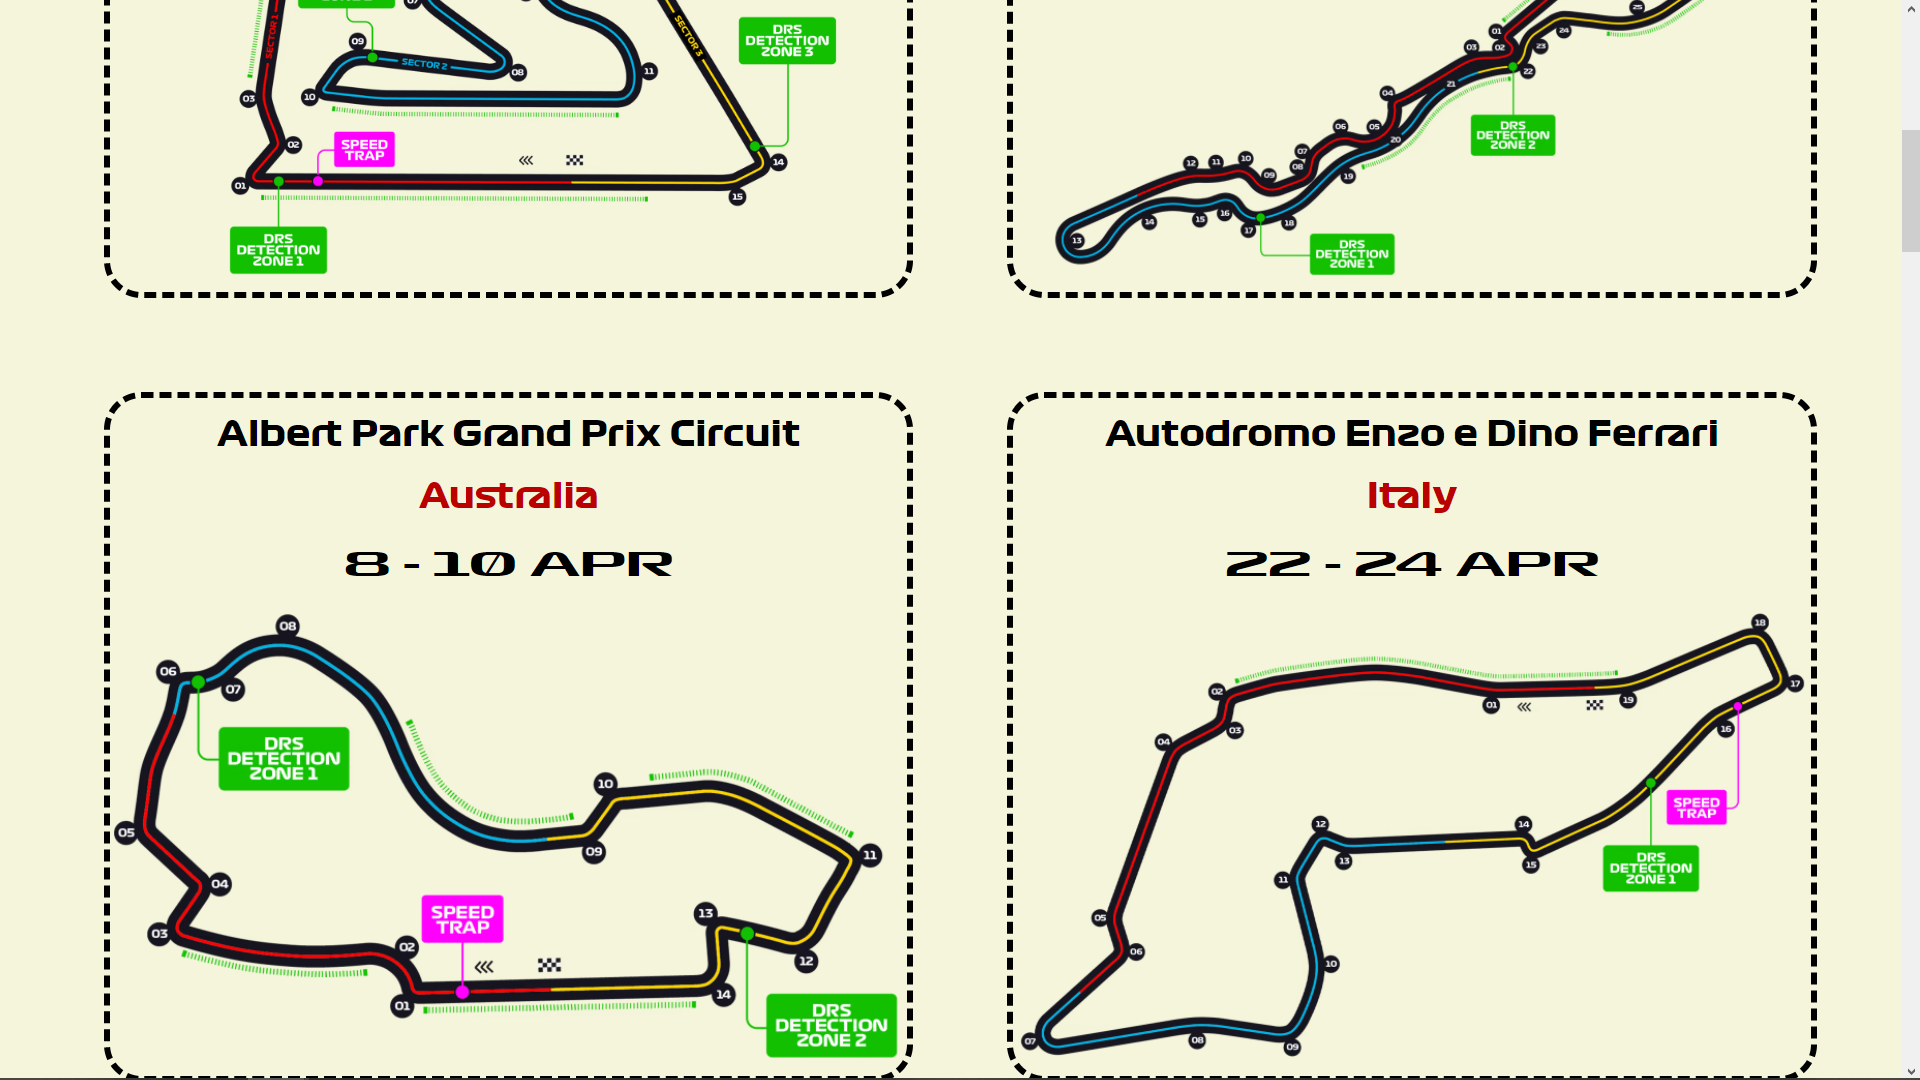
\includegraphics[scale=0.15]{images/schedule2} \\
	A versenynaptár & Görgetéssel látható az összes pálya
	\end{tabular}
	\caption{Versenynaptár}
	\label{abra:schedule}
\end{figure}

Ha átvisszük az egeret a kártya fölott, akkor mgejelenik egy gomb \textbf{Browse tickets} szöveggel, amelyre kattintva megtekinthetőek a versenyhez tartozó jegy típusok és azok információi (\ref{abra:ticketsUA}). Ha nincs bejelentkezve a felhasználó, akkor az \textbf{Add to cart} gomb szürkén jelenik meg, vagyis nem lehet a kosárba tenni, viszont ha rákattint a felhasználó, akkor a rendszer jelezni fogja egy \textbf{alert} (figyelmeztetés) ablakban, hogy autentikáció szükséges, ha ezt a funkciót szeretné használni.

\begin{figure}[!h]
	\centering
	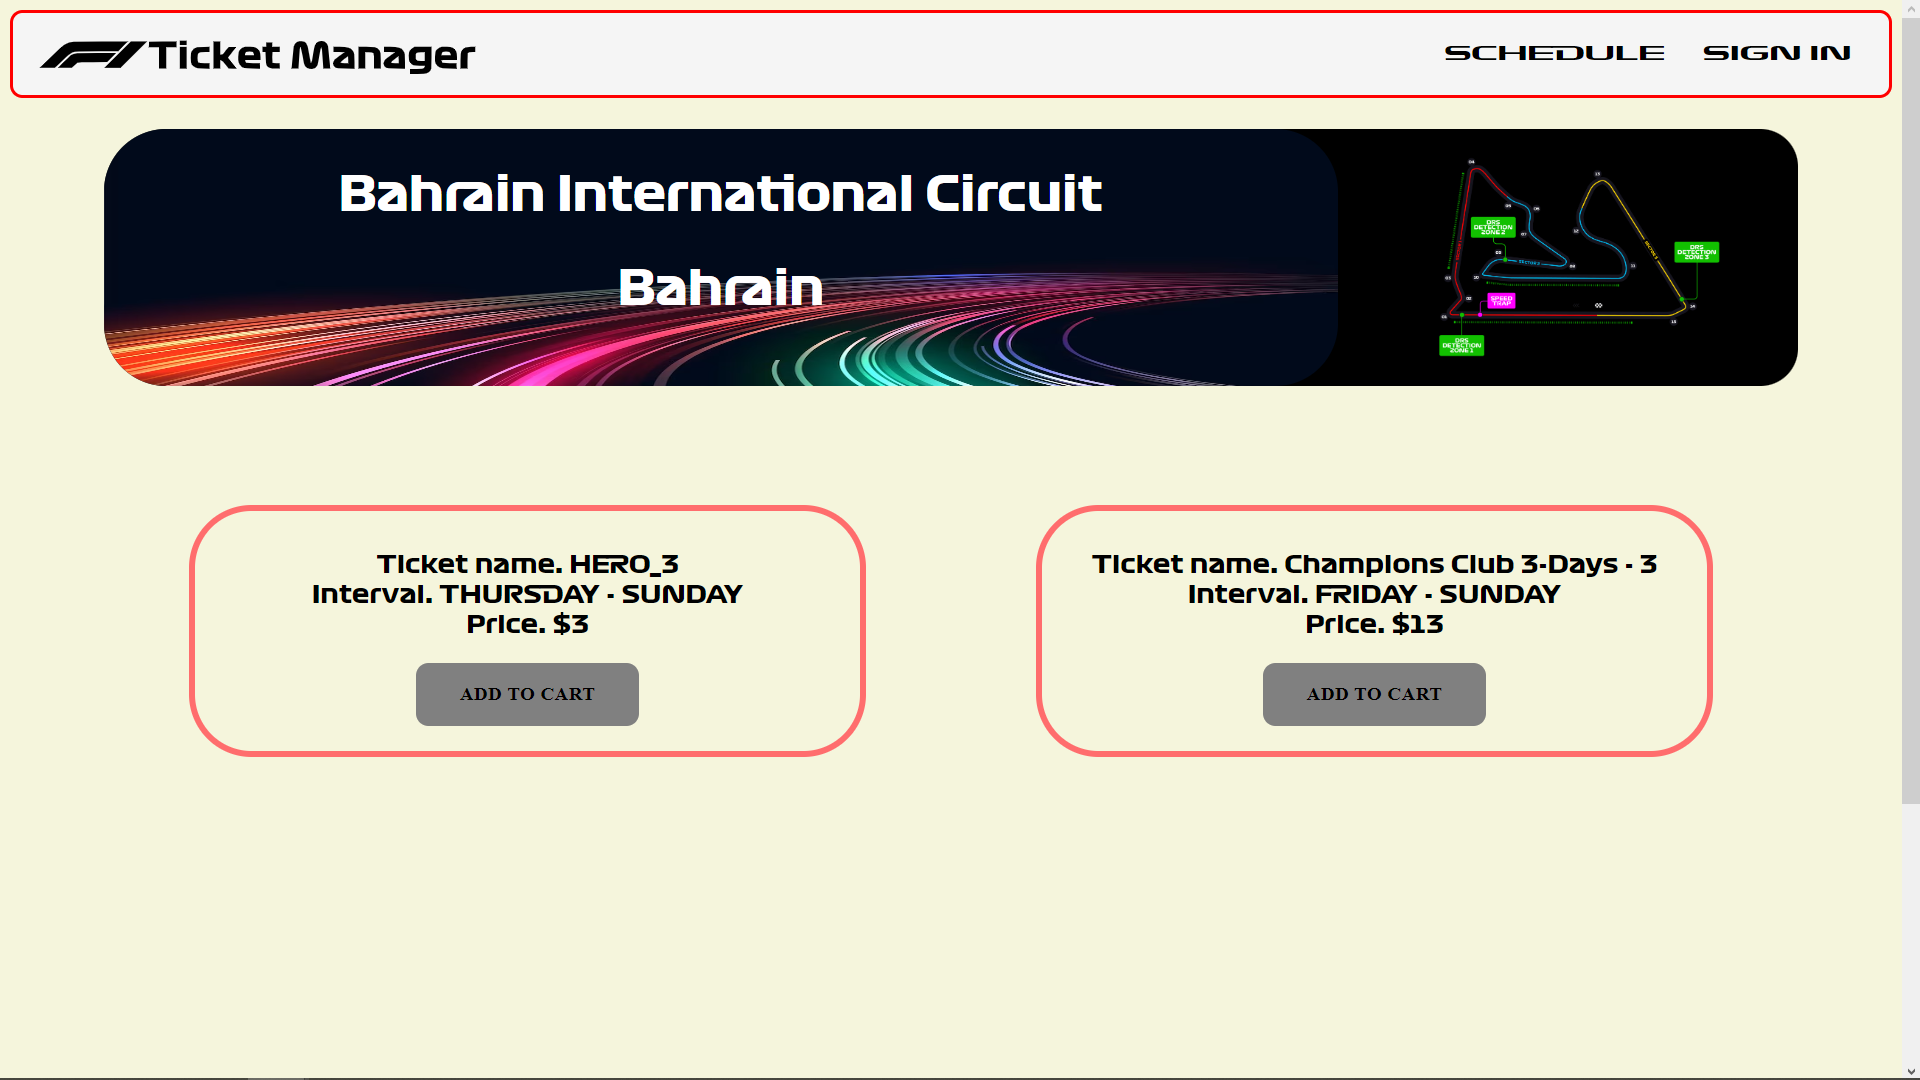
\includegraphics[scale=0.2]{images/tickets}
	\caption{Jegy típusok be nem jelentkezett felhasználóval}
	\label{abra:ticketsUA}
\end{figure}

Abban az esetben, ha a felhasználó be van jelentkezve, lehetőség van a jegyet a kosárba helyezni vagy visszajelzést adni az adott jegyről, élményekről (\ref{abra:ticketsAuth}). A jegyek mennyiségét a \textbf{Checkout} oldalon van lehetősége módosítani a felhasználónak. A rendszer ezen része egy továbbfejlesztési terület, hogy adott esetben ellenőrizve legyen, hogy tényleg csak az tudjon visszajelzést adni, akkor vásárolt az adott jegyből. 

\begin{figure}[!h]
	\centering
	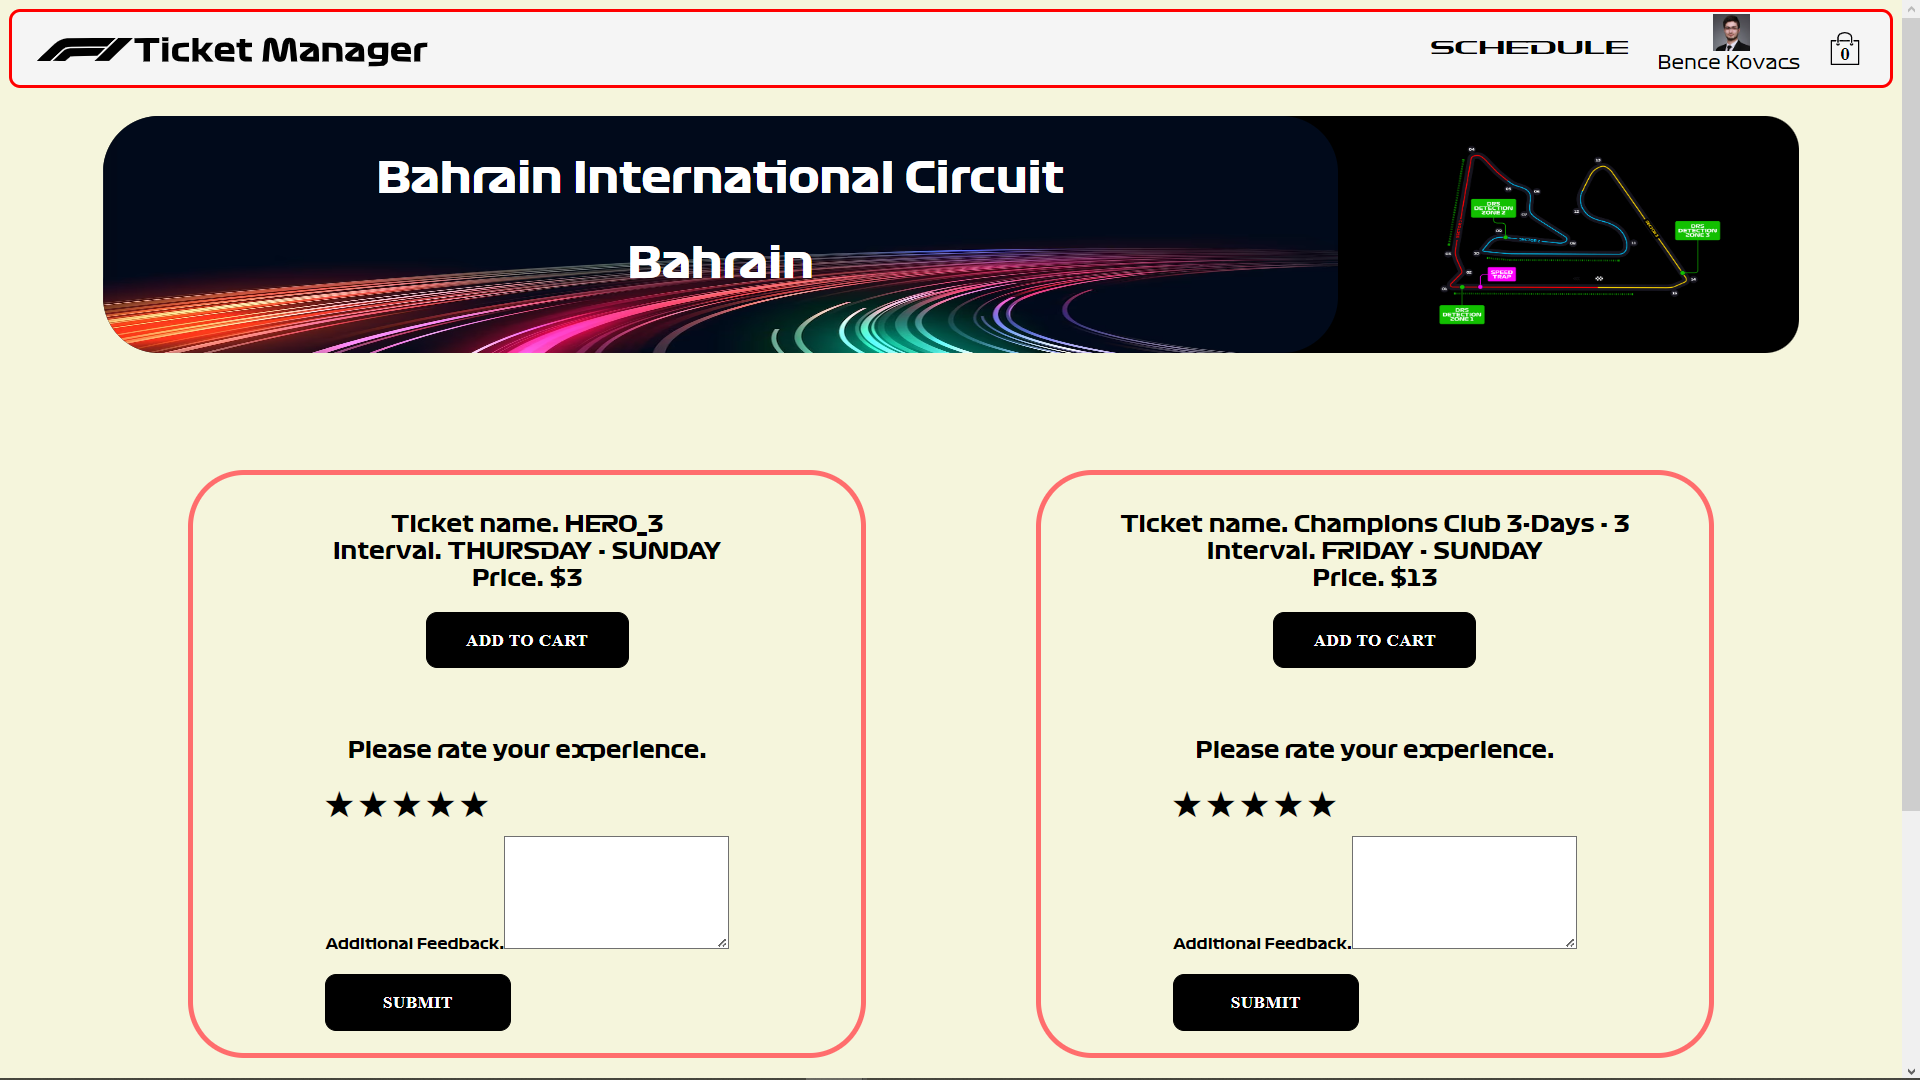
\includegraphics[scale=0.2]{images/ticketsAuth}
	\caption{Jegy típusok bejelenkezett felhasználóval}
	\label{abra:ticketsAuth}
\end{figure}

\subsection {Bejelentkezés és regisztráció (Sign in and up)}

A bejelentkezési felületen egyben lett feltüntetve a bejelentkezés és regisztráció két külön kártyán. Az email címmel vagy közösségi fiókkal való autentikáción kívül lehetőség van elfelejtett jelszó esetén új megadása. Ennek érdekében a felhasználó megadja az email címét és kapni fog egy levelet, amely tartalmaz egy linket az új jelszó megadásához (\ref{abra:signInUp}).

\begin{figure}[!h]
	\centering
	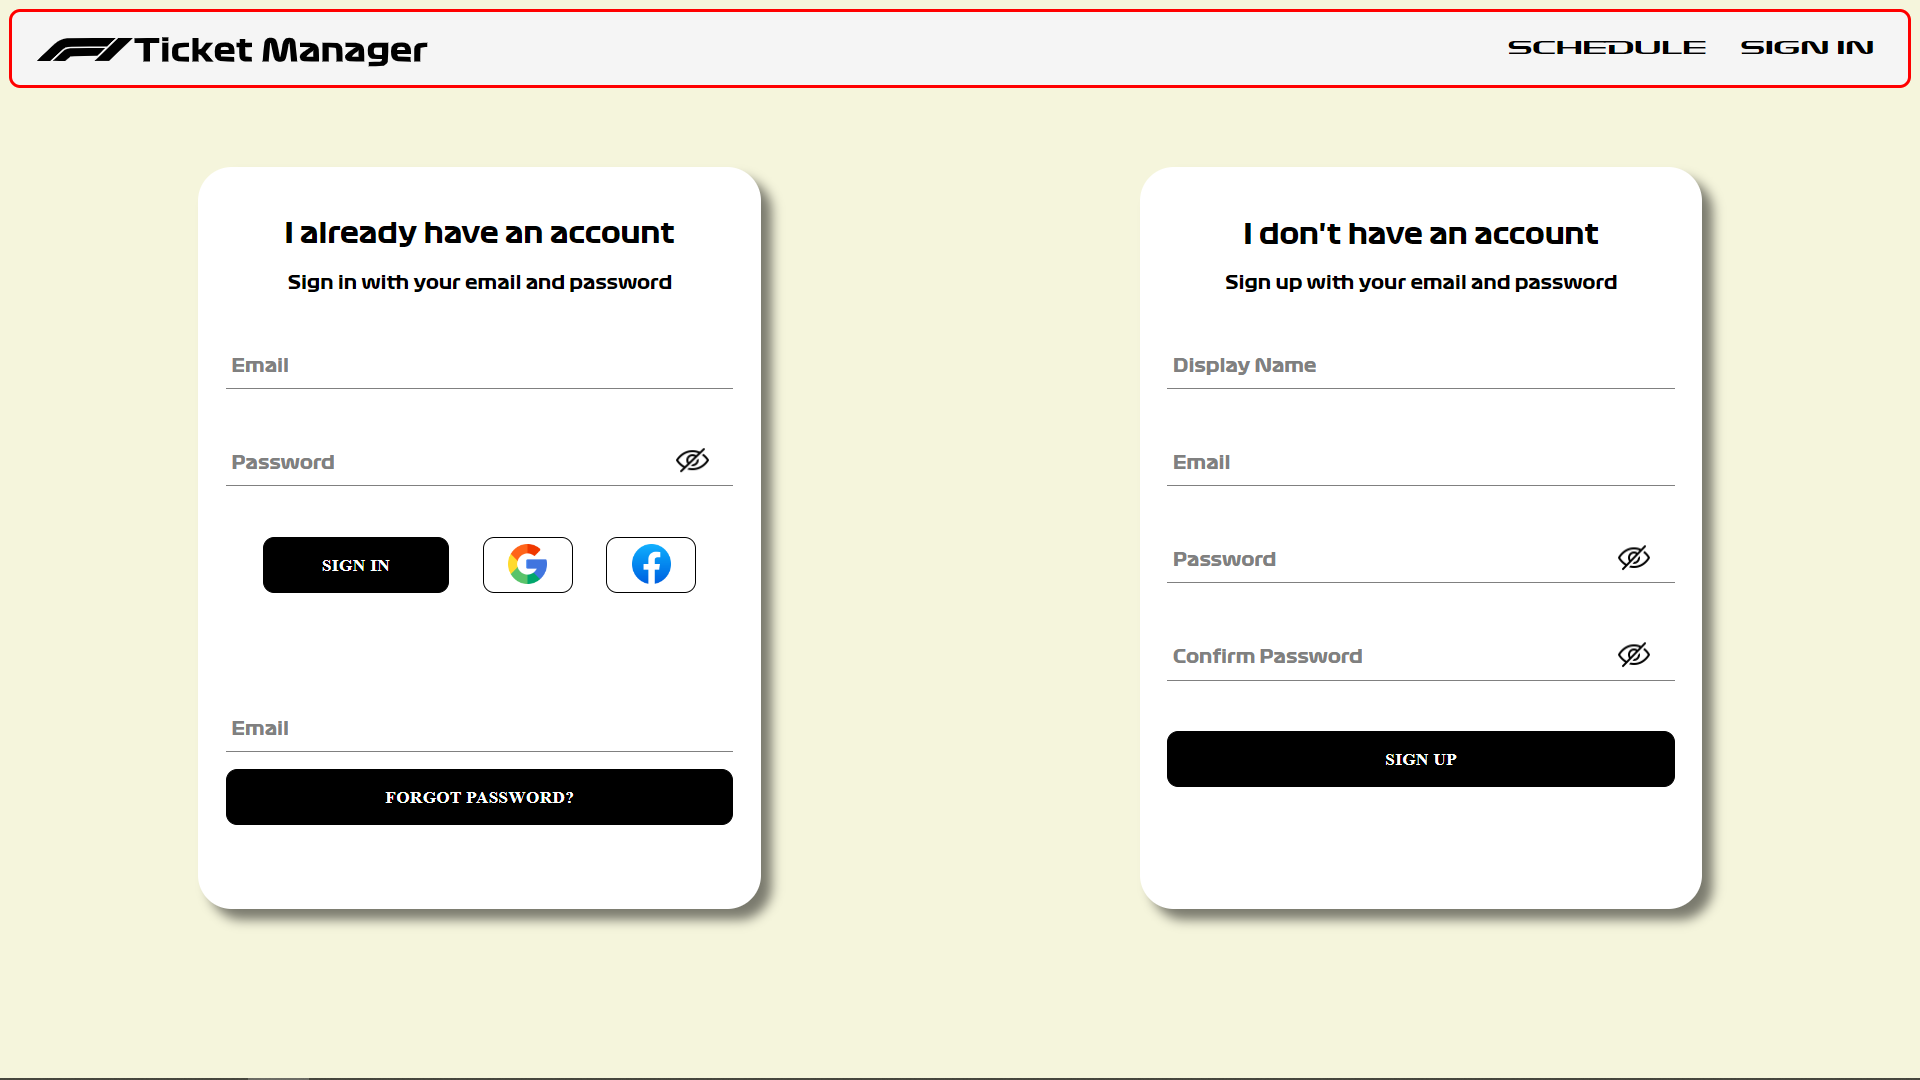
\includegraphics[scale=0.2]{images/signInUp}
	\caption{Autentikáció}
	\label{abra:signInUp}
\end{figure}

Továbbá lehetőség van a felületre való regisztrációra is a jobb oldali kártyán. Ennek a folyamatnak a bemutatására készítettem egy szekvencia diagramot a \textbf{SequenceDiagram.org} online szerkesztő segítségével \cite{Seq}.

\begin{figure}[!h]
	\centering
	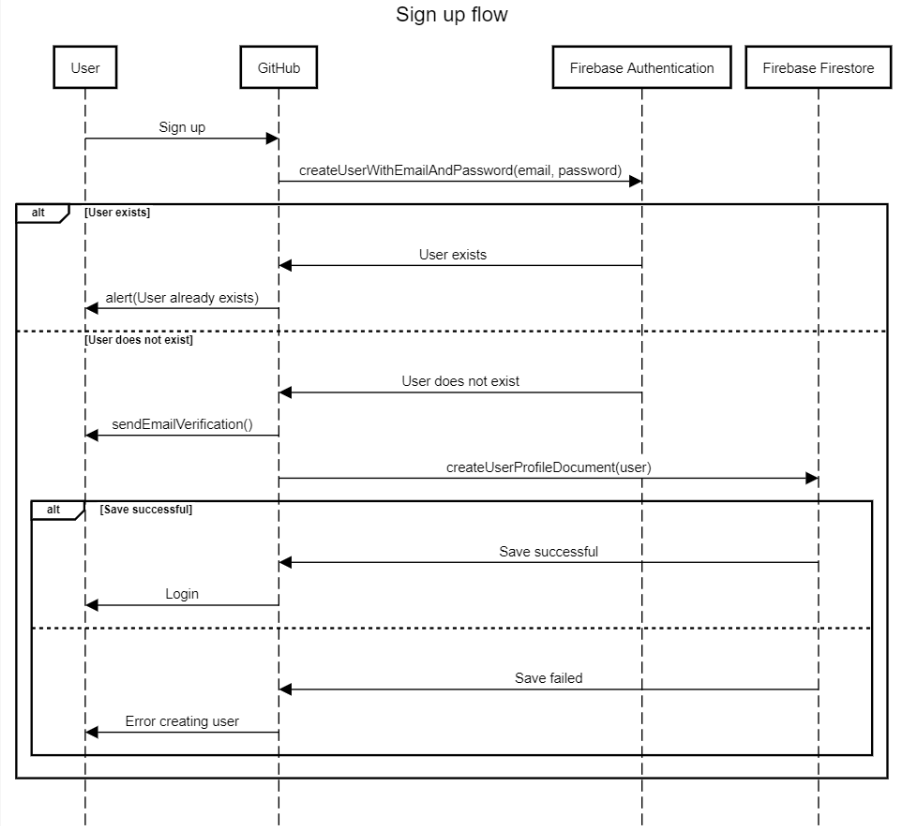
\includegraphics[scale=0.5]{images/signUpFlow}
	\caption{Szekvencia diagram - Regisztráció}
	\label{abra:signUpFlow}
\end{figure}
\pagebreak

A regisztráció folyamatát a felhasználó indítja el a kötelező mezők kitöltésével és a gomb megnyomásával. A \textit{Firebase} szerver első sorban ellenőrzni, hogy az adott email címmel már létezik-e felhasználó és amennyiben igen, a megfelelő üzenetet jeleníti meg az oldal. Ellenkező esetben létrehozza a rendszerben a felhasználót, elmenti a megadott adatokat egyéb meta adatokkal kiegészítve, mint a létrehozás dátuma. A mentés után a rendszer automatikusan be is jelentkezteti a felhasználót (\ref{abra:signUpFlow}).

\subsection {Profil (Profile)}

A \textbf{Profil} oldal elérése csak a bejelentkezett felhasználóval lehetséges (\ref{abra:profile}). Ezen az oldalon lehetséges a profilkép és a megjelenített név módosítása az \textbf{Edit profile} gombra kattintva.

\begin{figure}[!h]
	\centering
	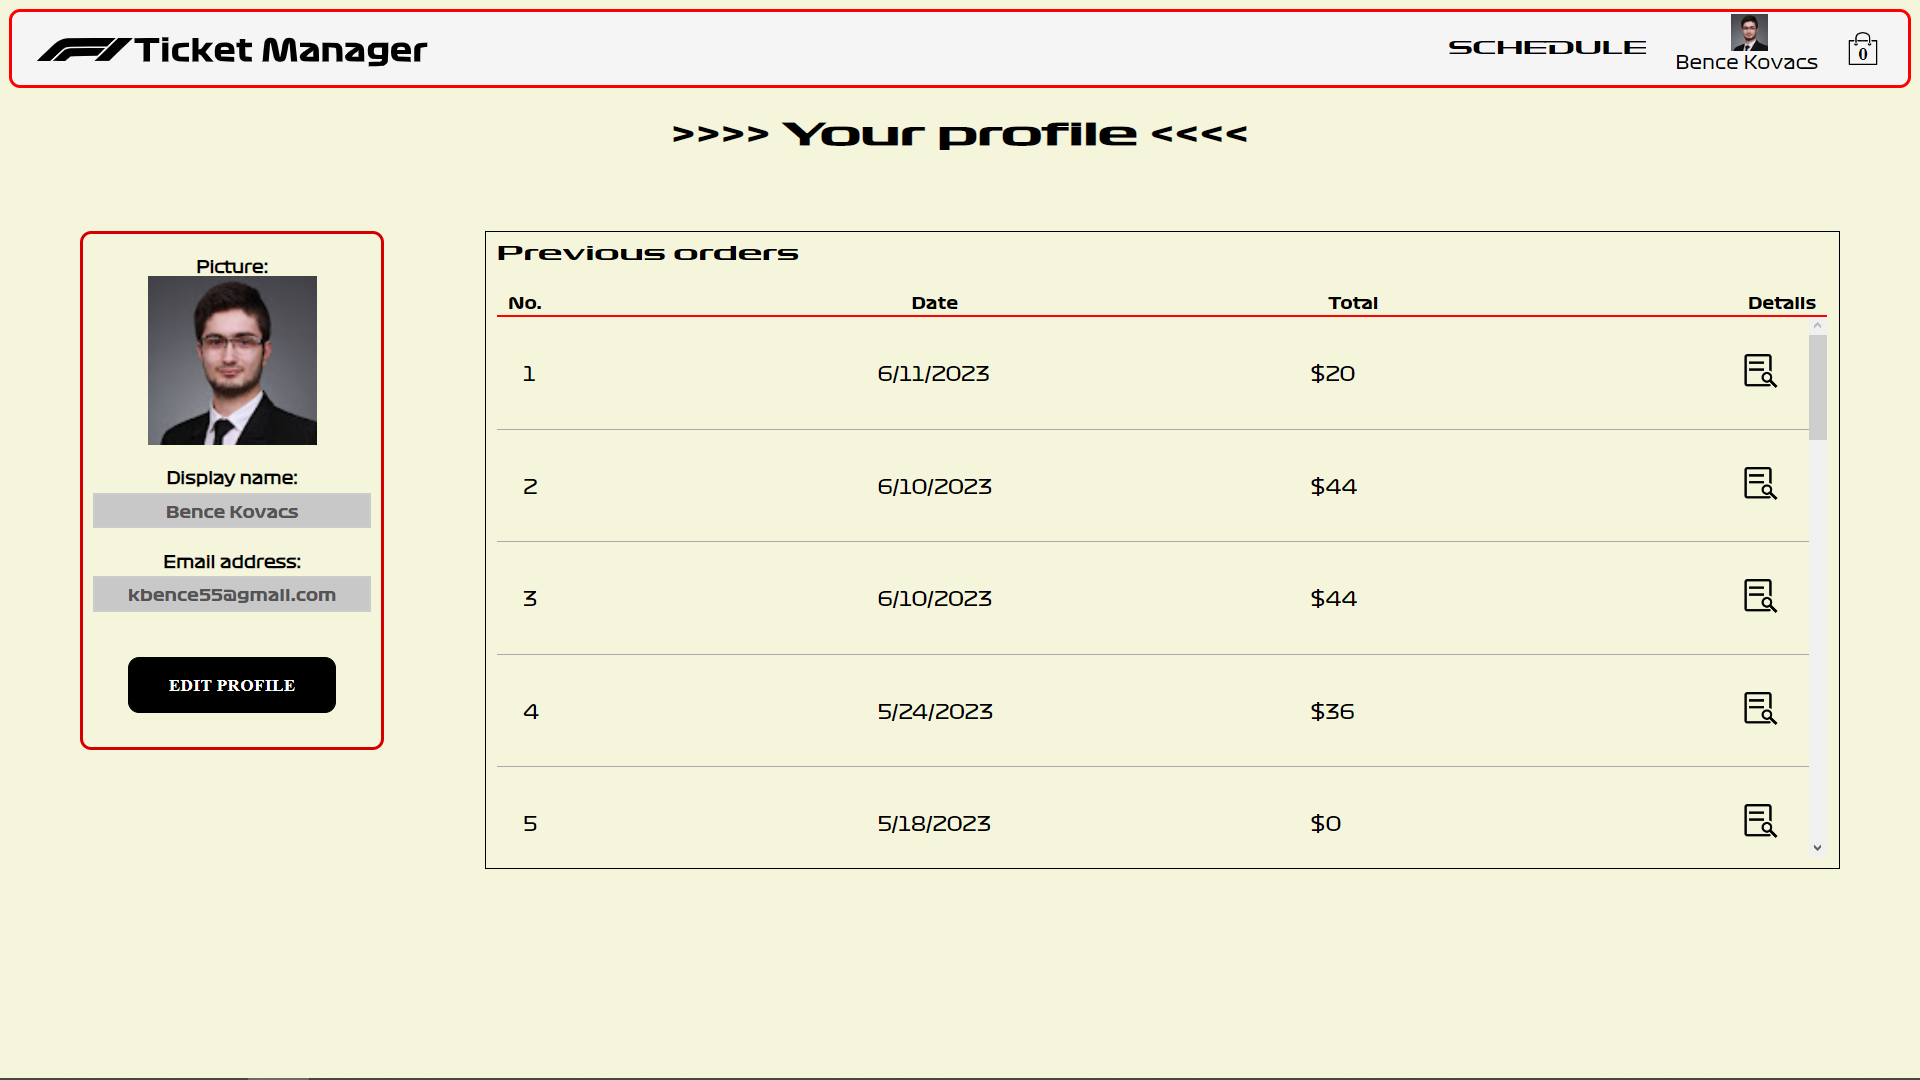
\includegraphics[scale=0.2]{images/profile}
	\caption{Saját profil oldal}
	\label{abra:profile}
\end{figure}

Az oldal jobb részén láthatóak a \textbf{rendelési előzmények}. Ezek görgetéssel böngészhetőek és a jobb szélén levő ikonra kattintva tekinthetőek meg a vásárlás részletei (\ref{abra:previousOrders}).

\begin{figure}[!h]
	\centering
	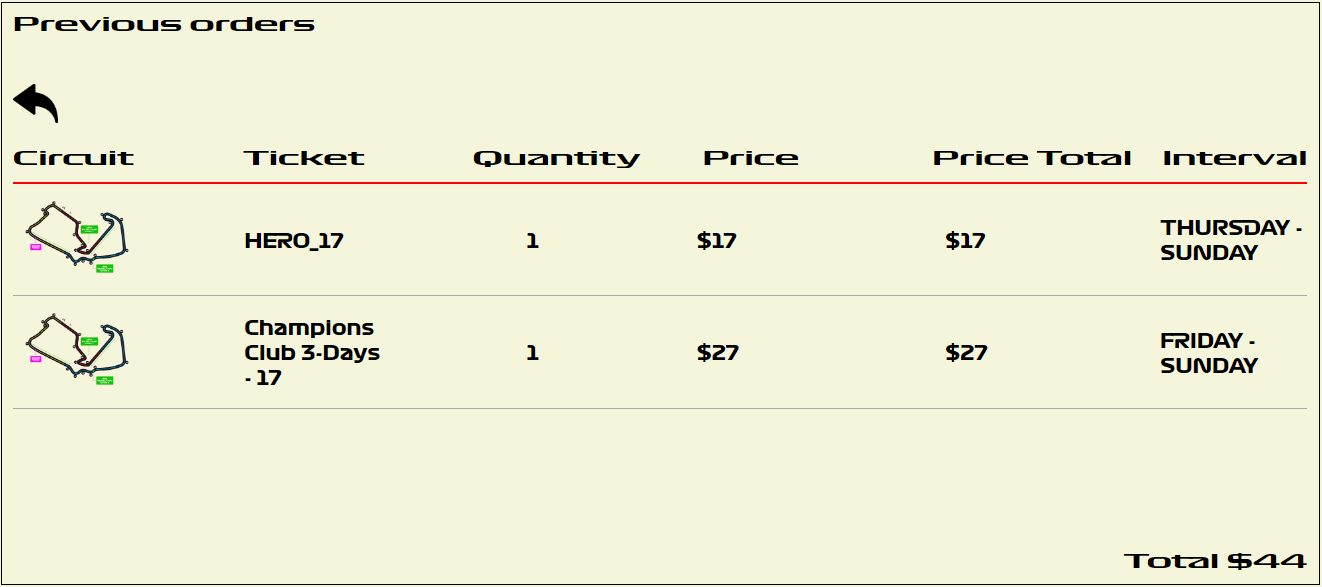
\includegraphics[scale=0.3]{images/previousOrders}
	\caption{Rendelés részletei}
	\label{abra:previousOrders}
\end{figure}

Amennyiben elvisszük valamely elem fölött az egeret megjelenik egy \textbf{More details} gomb, amelyre kattintva megtekinthető a jegy egyedi azonosítója (\ref{abra:moreDetails}). Ez a funkcionalitás azért fontos, mivel megtörténhet, hogy a felhasználó elveszíti vagy nem kapja meg a QR kódot emailben, ami ezt az azonosítót tartalmazza. Ha ez bekövetkezne, akkor innen is lehetőség van kimásolni és a megszokott módon azonosítani a PIN kóddal.

Ezen a felugró ablakon továbbá lehetősége van a felhasználónak egy új PIN kódot megadni, ha a meglévő elfelejtette vagy úgy érzni, hogy valaki megszerezhette. Ezután egy újabb felugró ablakban lehetséges a PIN kód megváltoztatása. 

\begin{figure}[!h]
	\centering
	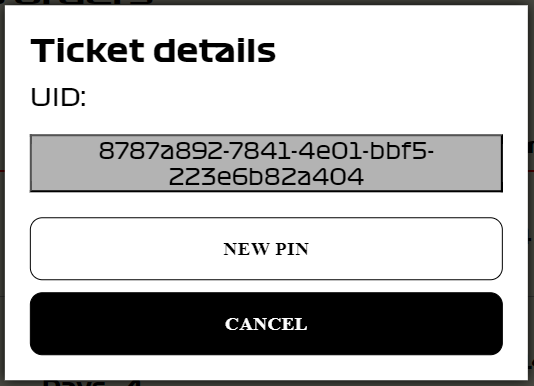
\includegraphics[scale=0.4]{images/moreDetails}
	\caption{Jegy részletei}
	\label{abra:moreDetails}
\end{figure}

A PIN kód megadásánál kötelezően egy 6 számjegyű számot kell megadni (\ref{abra:pinPopup}). Ezt manuálisan is be lehet írni vagy a \textit{pálca} ikonra kattintva generálódik egy véletlenszerű szám. A \textbf{Submit} gombra kattintva frissítheti a felhasználó a jegyhez tartozó kódot, ami teljes mértékben felülírja az előzőt, ezért nagyon figyelmes kell lenni a megadásakor, de erre a pirossal írt szöveg is figyelmezteti a vásárlót.

\begin{figure}[!h]
	\centering
	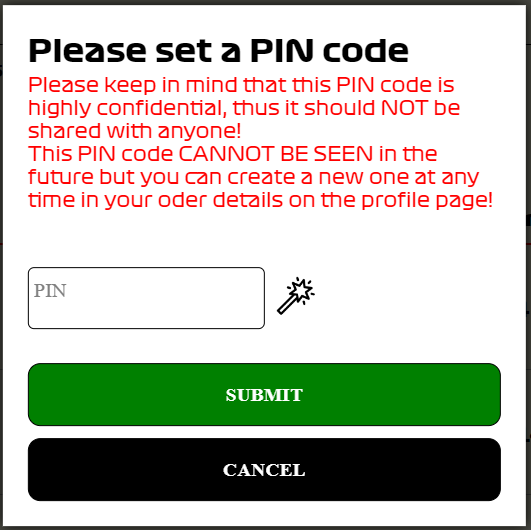
\includegraphics[scale=0.4]{images/pinPopup}
	\caption{PIN kód megadása}
	\label{abra:pinPopup}
\end{figure}
\pagebreak

\subsection {Rendelés (Checkout)}

A \textbf{Rendelés} oldalon van lehetősége a felhasználónak véglegesíteni a vásárlást (\ref{abra:checkout}). Itt is láthatóak a kosárba helyezett jegyek információi és csak itt módosíthatóak az egyes jegyek mennyisége vagy a kosárból való törlése. A \textbf{Pay Now} gombra kattintva tud a felhasználó végig lépkedni a fizetési, a számlázási adatok kitöltésén és végül véglegesíteni a vásárlást. Sikeres vásálás esetén a felhasználónak küld a rendszer egy emailt, amiben megkapja a vásárlási információkat és QR kódokat. Az emailek küldésére a \textbf{Brevo} szolgáltatót vettem ígénybe \cite{Brevo}.

\begin{figure}[!h]
	\centering
	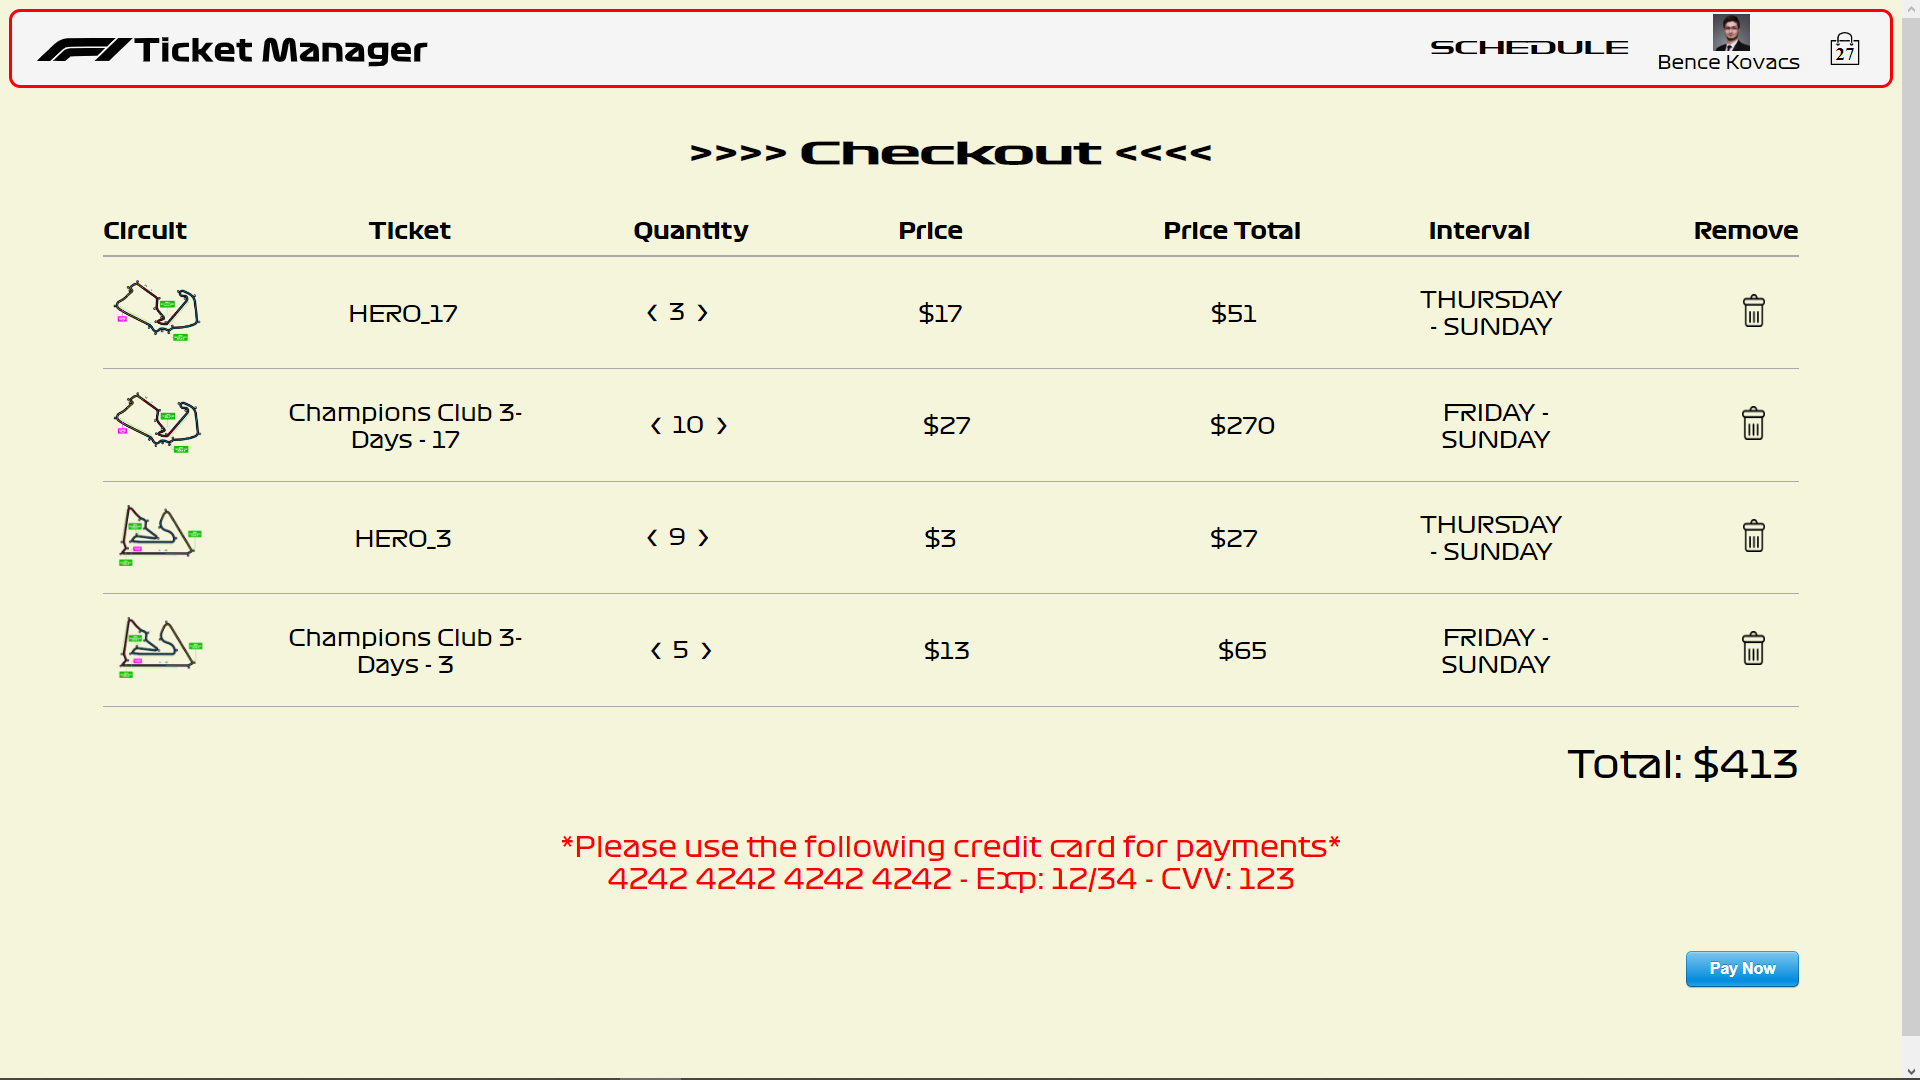
\includegraphics[scale=0.2]{images/checkout}
	\caption{Rendelés véglegesítése}
	\label{abra:checkout}
\end{figure}

\pagebreak
\subsection {Beléptetés (Scan)}

A \textbf{Beléptetés} oldalon a rendszer \textit{Adminisztrátora(i)} tudják a jegyeket hitelesíteni a versenyhelyszíneken az erre a célra kihelyezett termináloknál (\ref{abra:scan}). A felhasználó a kamera elé helyezi a QR kódot \cite{RQR}, majd beírja a PIN kódot, amelyeket a rendszer rögzít és jelzi a hitelesítési folyamat eredményét.

\begin{figure}[!h]
	\centering
	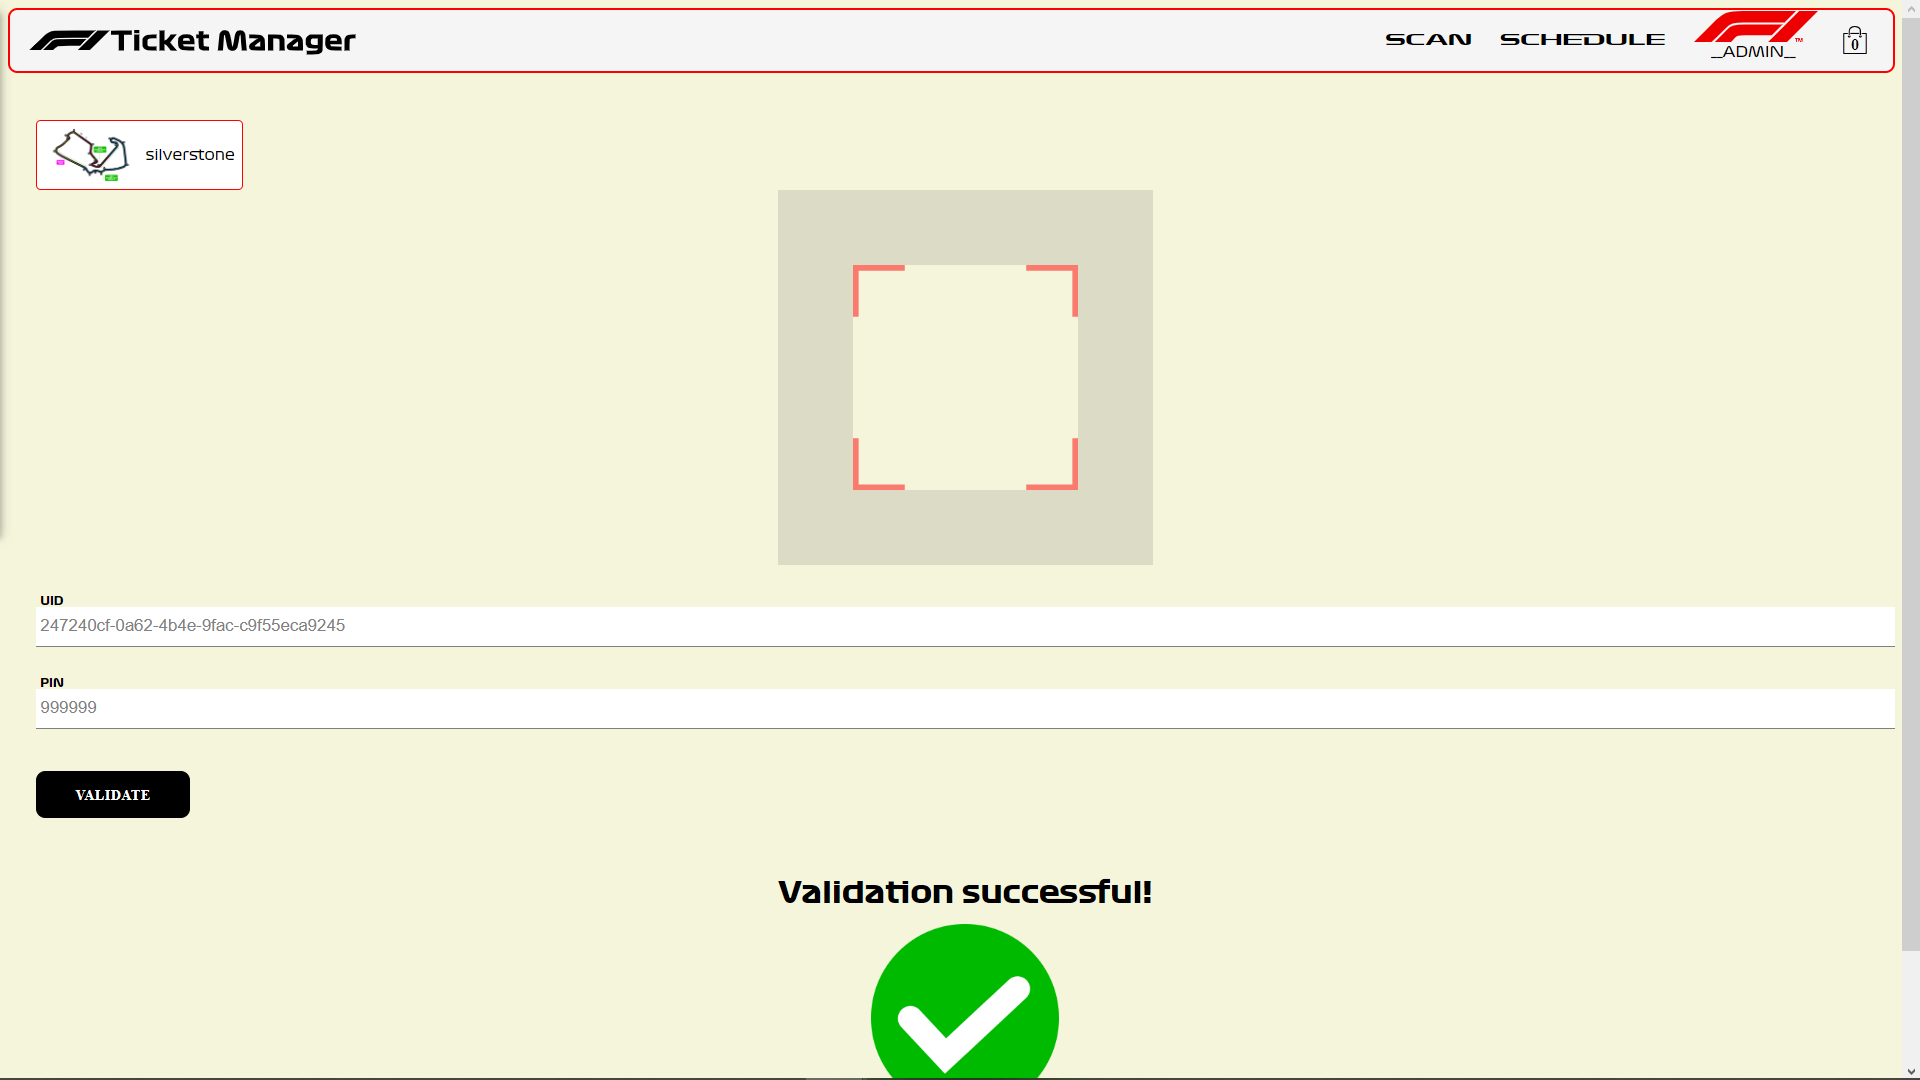
\includegraphics[scale=0.2]{images/scan}
	\caption{Jegyek hitelesítése}
	\label{abra:scan}
\end{figure}